\chapter{Manta Flow platform}

Before we get into the details of data lineage analysis service for embedded code, let us first introduce and describe Manta Flow platform. It is the platform that the service is integrated with and influences many of the design and implementation decisions. It also provides a couple of solution examples for problems we face that we will use for inspiration.

%---------------------
% SECTION
%---------------------
\section{Manta Flow overview}

Manta Flow is an automated data lineage platform that scans data environments to build and visualize a graph of all data flows (as seen in figure~\ref{fig01:lineage}) within it. This graph enables its users to get better visibility and control of their data processes. The emphasis is on \textit{automation}, Manta Flow requires little intervention apart from configuration and can perform data lineage analysis in a matter of hours to days, compared to manual analysis which can take weeks to months, so the visualization provides up-to-date information.
\par
Data lineage analysis is based on the analysis of metadata and scripts extracted from the connected systems. Metadata contain information about schema and structure of internal entities and their relations. Scripts contain data processing and transformation logic on these entities. It is not possible to construct complete data lineage from just one of these sources.
\par
Manta Flow is made up of three major components.
\begin{itemize}
    \item \textit{Manta Flow CLI} is a Java command line application that extracts all metadata and scripts from source data technologies, analyzes them, sends all gathered metadata to the \textit{Manta Flow Server}, and optionally, processes and uploads the generated export to a target metadata database.
    \item \textit{Manta Flow Server} is a Java server application that stores all gathered metadata inside its metadata repository, transforms it to a form suitable for import to a target metadata database, and provides it to its visualization or third-party applications via API.
    \item \textit{Manta Admin UI} is a Java server application providing a graphical and programming interface for installation, configuration, updating, and overall maintenance of Manta Flow.
\end{itemize}
\par
Each data environment consists of a different set of data technologies. Each data technology stores its internal data in a different metadata structure and provides a different API to access it. In order to be able to analyze the entire environment, Manta Flow CLI uses a wide range of proprietary scanners, currently there are over 40. Each scanner can connect to and analyze data lineage for a single data technology to accommodate its specific structure. It produces a common metadata output uploaded to Manta Flow Server's repository. This architecture allows an easier support of a new data technology by developing a new scanner.

\begin{figure}[ht]\centering
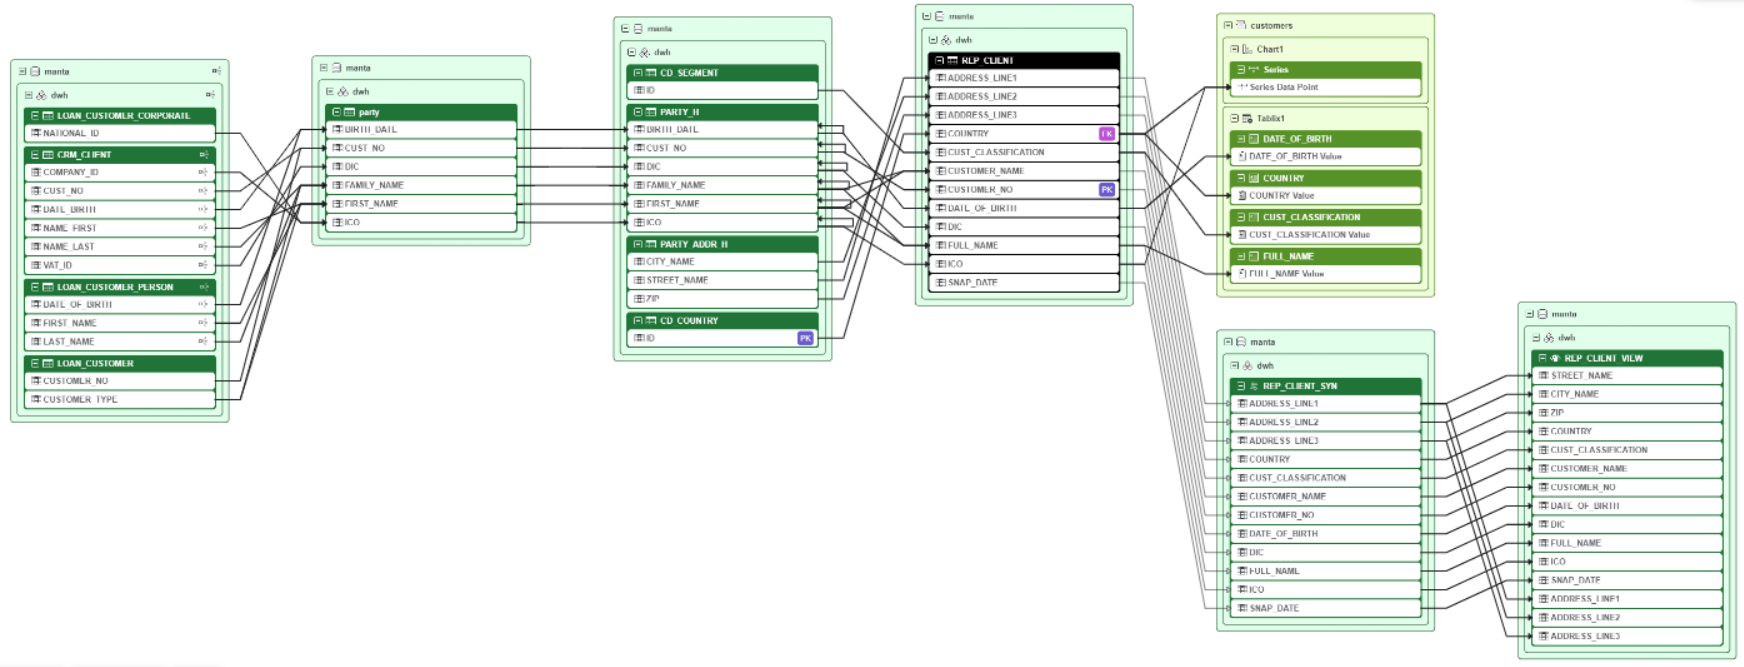
\includegraphics[width=1.0\textwidth]{img/lineage_example.PNG}
\caption{An example of data lineage visualization in Manta Flow}
\label{fig01:lineage}
\end{figure}  

%---------------------
% SECTION
%---------------------
\section{Manta graph}

The common output of all scanners is a data structure called \textit{Manta graph}. It allows to capture both data environment structure and data flows within it. A graph consists of nodes (vertices) and edges between them. A node may represent a data source or a transformation, e.g., a database table column, a report dimension or a union of columns. Edges are directed and represent data flow from one node to the other.
\par
Nodes have a layered structure to allow representation of a logical hierarchy. This is expressed in a child-parent relationship between nodes, e.g., a server node could be a parent to several database nodes, each database node would have table node children and in each table there would be column node children. However, only the nodes on the lowest level can be connected with data flow edges. This hierarchy is important for visualization to simplify grouping of related nodes such as all columns of a table and to define node paths.
\par
Each node is identified by a unique path derived from its name and names of its parent nodes, which enables merging the same entity and associated data flows in different graphs. For example, if an MSSQL database table is a source of a view in that same database and is also used in a report in SSRS reporting tool, it will be created with the same identification in MSSQL scanner output and in SSRS scanner output. Manta Flow Server is then able to merge these outputs to visualize one node with two distinct data flows. This can be seen in figure~\ref{fig01:lineage} where SSRS nodes are framed in a different shade of green than those belonging to MSSQL.

%---------------------
% SECTION
%---------------------
\section{Scanners}

Scanners are important building blocks of Manta Flow. The role of a scanner is to analyze data lineage in systems of a particular data technology. Ins and outs of each data technology are different, so each scanner does its job in a different way, but they all have a similar structure. They consist of two main components, a \textit{Connector} and a \textit{Dataflow Generator}.

\subsection{Connector}

The purpose of a \textit{Connector} component is to facilitate a connection to the analyzed resource and prepare metadata for analysis. That consists of two steps, metadata extraction and creating a general model from the extracted metadata. 

\subsubsection{Extractor}

Metadata extraction is performed by an \textit{Extractor} sub-component of a Connector. The goal is to connect to the analyzed system using the configured connection options (URL, credentials or access tokens) and extract all metadata required for the dataflow analysis. The metadata can contain information such as database schema, definition of reports with all dimensions and facts that are used in them or enumeration of ETL pipelines with their sources, destinations and individual transformations. Other artifacts could be extracted, too, such as scripts of any kind, configuration etc. All extracted resources are stored locally in one place so that the analysis can be executed in \textit{offline} mode, that is, without requiring an active connection to any other system. The format in which they are stored is not important, however most often the format of raw extracted metadata is used.
\par
Database scanners usually go one step further and create so called \textit{data dictionary} from the extracted metadata. Data dictionary stores schema of extracted database resources in a universal data structure that is able to capture different hierarchical structure. It is a kind of pre-processing so this information can be used by readily used by other scanners in the later stages of the analysis should they need it. Extraction is always executed before other stages of data flow analysis for all scanners. 

\subsubsection{Reader}

The other sub-component of a Connector is called \textit{Reader}. Its purpose is to read extracted metadata and create a universal model that can be used for data flow analysis. This model serves as an interface between a Connector and a Dataflow Generator. It helps to create an abstraction of metadata, because its format or the way it is read may change in time.

\subsection{Dataflow Generator}

Dataflow Generator discovers data flows in target systems using the extracted inputs. The output of such analysis is a Manta graph. There are multiple steps in this process and the specifics vary between different scanners. Usually it in includes translating structured metadata into nodes and edges following data flow rules. Suppose that we have created a report in a tool such as Tableau. We used a database view as our data source and we visualized one of the columns as a dimension in the report. Furthermore, we computed another dimension from two other columns. Dataflow Generator would create nodes for the view columns, nodes for the dimensions in the report and then add edges between the columns and dimensions.
\par
Database scanners also analyze queries and scripts present in databases. There are Data Definition Language (DDL) scripts which define database objects (tables, views, triggers, stored procedures etc.). Analyzing them is more complicated than creating data flows based on metadata. The algorithm for processing database queries and scripts is based on parsing a well-defined language. For example, a database view is created from a database query, so first, the query is resolved, the columns of the tables included in the query are created and then connected with the corresponding view columns.

% Description of query service, how it works, similarities to what we are trying to achieve.
%- it has a common interface
%- usually used when the connection details are not entirely known
%- could also be that nothing is known
%- can deduce
%- only resolves queries for which it constructs nodes
%---------------------
% SECTION
%---------------------
\section{Dataflow Query Service}

Sometimes, a scanner for one data technology runs into a database query that defines a data source. It is a common feature of many reporting and analytic tools. It would not make sense to include a support for each SQL dialect in all such scanners, firstly because it is quite complicated, but also because there are scanners that can process it already. Furthermore, there might not be enough information in the context of this scanner to resolve such query. Take for example a query \texttt{SELECT * FROM TABLE\_A}. The scanner doesn't know the columns present in \texttt{TABLE\_A}, so it is not possible to provide an accurate representation. 
\par
\textit{Dataflow Query Service} is a component that was introduced to help with processing of embedded SQL queries. It provides a unified service interface that allows launching execution of a database scanner on a small input that can be used by other data technologies. It works by selecting the appropriate scanner for the provided input, executing data flow analysis and merging the resulting sub-graph into the graph of the original data technology scanner.
\par
One of the main benefits of this service is that it uses data dictionaries created by each scanner in the extraction phase, therefore it has access to extracted database schemas, which allows it to resolve exact columns for queries such as \texttt{SELECT * FROM TABLE\_A}. It is also useful in situations when details about the target systems are unknown or unresolved, the service has the ability to deduce columns from available information and to choose the appropriate scanner from the provided connection details.

\subsubsection{Overview}
In general, there are three pieces of information needed to analyze an SQL query:
\begin{itemize}
    \item Connection data - connection type, connection string, server hostname (at least connection string or server name is needed).
    \item Default data - default database, default schema, connecting user (as applicable) in case connection data is not available or not recognized.
    \item Query or embedded script text.
\end{itemize}
If the data technology scanner has all of the above information, it constructs a \texttt{Connection} object directly, otherwise it is expected to perform connection mapping by retrieving the required data from manual configuration. Connection and query text are inputs for Dataflow Query Service. Next, dictionary mapping is performed, that is, an appropriate target scanner and a persisted data dictionary is selected based on \texttt{Connection} data. The selected scanner is invoked with query text, data dictionary and defaults, which provides the result in form of a \texttt{DataflowQueryResult}. The data technology then uses this result to connect the resulting lineage to the relevant nodes in the host script and to merge the result into the main graph.

\subsubsection{External connections}
One of the main purposes of \texttt{DataflowQueryResult} is to perform connection to external nodes. The purpose of embedded queries is to provide data for further processing, therefore we would like to connect the nodes of the query objects with other nodes in the lineage, e.g., connect database columns with data fields in a report. These connection points are unknown to the query scanner and the host scanner doesn't understand the query in advance, so the result graph contains extra nodes called \textit{pin} nodes.
\par
Pin nodes represent an input to a node representing query parameter or an output from a query resultset column. After the query is analyzed and its graph is created, the service adds these pin nodes and connects them with appropriate edges to the result nodes. Then, the host scanner might provide a mapping from pin nodes to nodes in the host graph. The service creates new edges from pin nodes to host graph nodes (and vice versa, depending on the direction) based on the provided mapping and then contracts the pin nodes, thus effectively connecting the resultset column node or a parameter node with the host graph node. Should any pin node remain unmatched, it is filtered out in filtering task later in the scenario.

\subsubsection{Architecture}
%%% copied from Confluence, can I somehow quote this?
\begin{figure}[ht]\centering
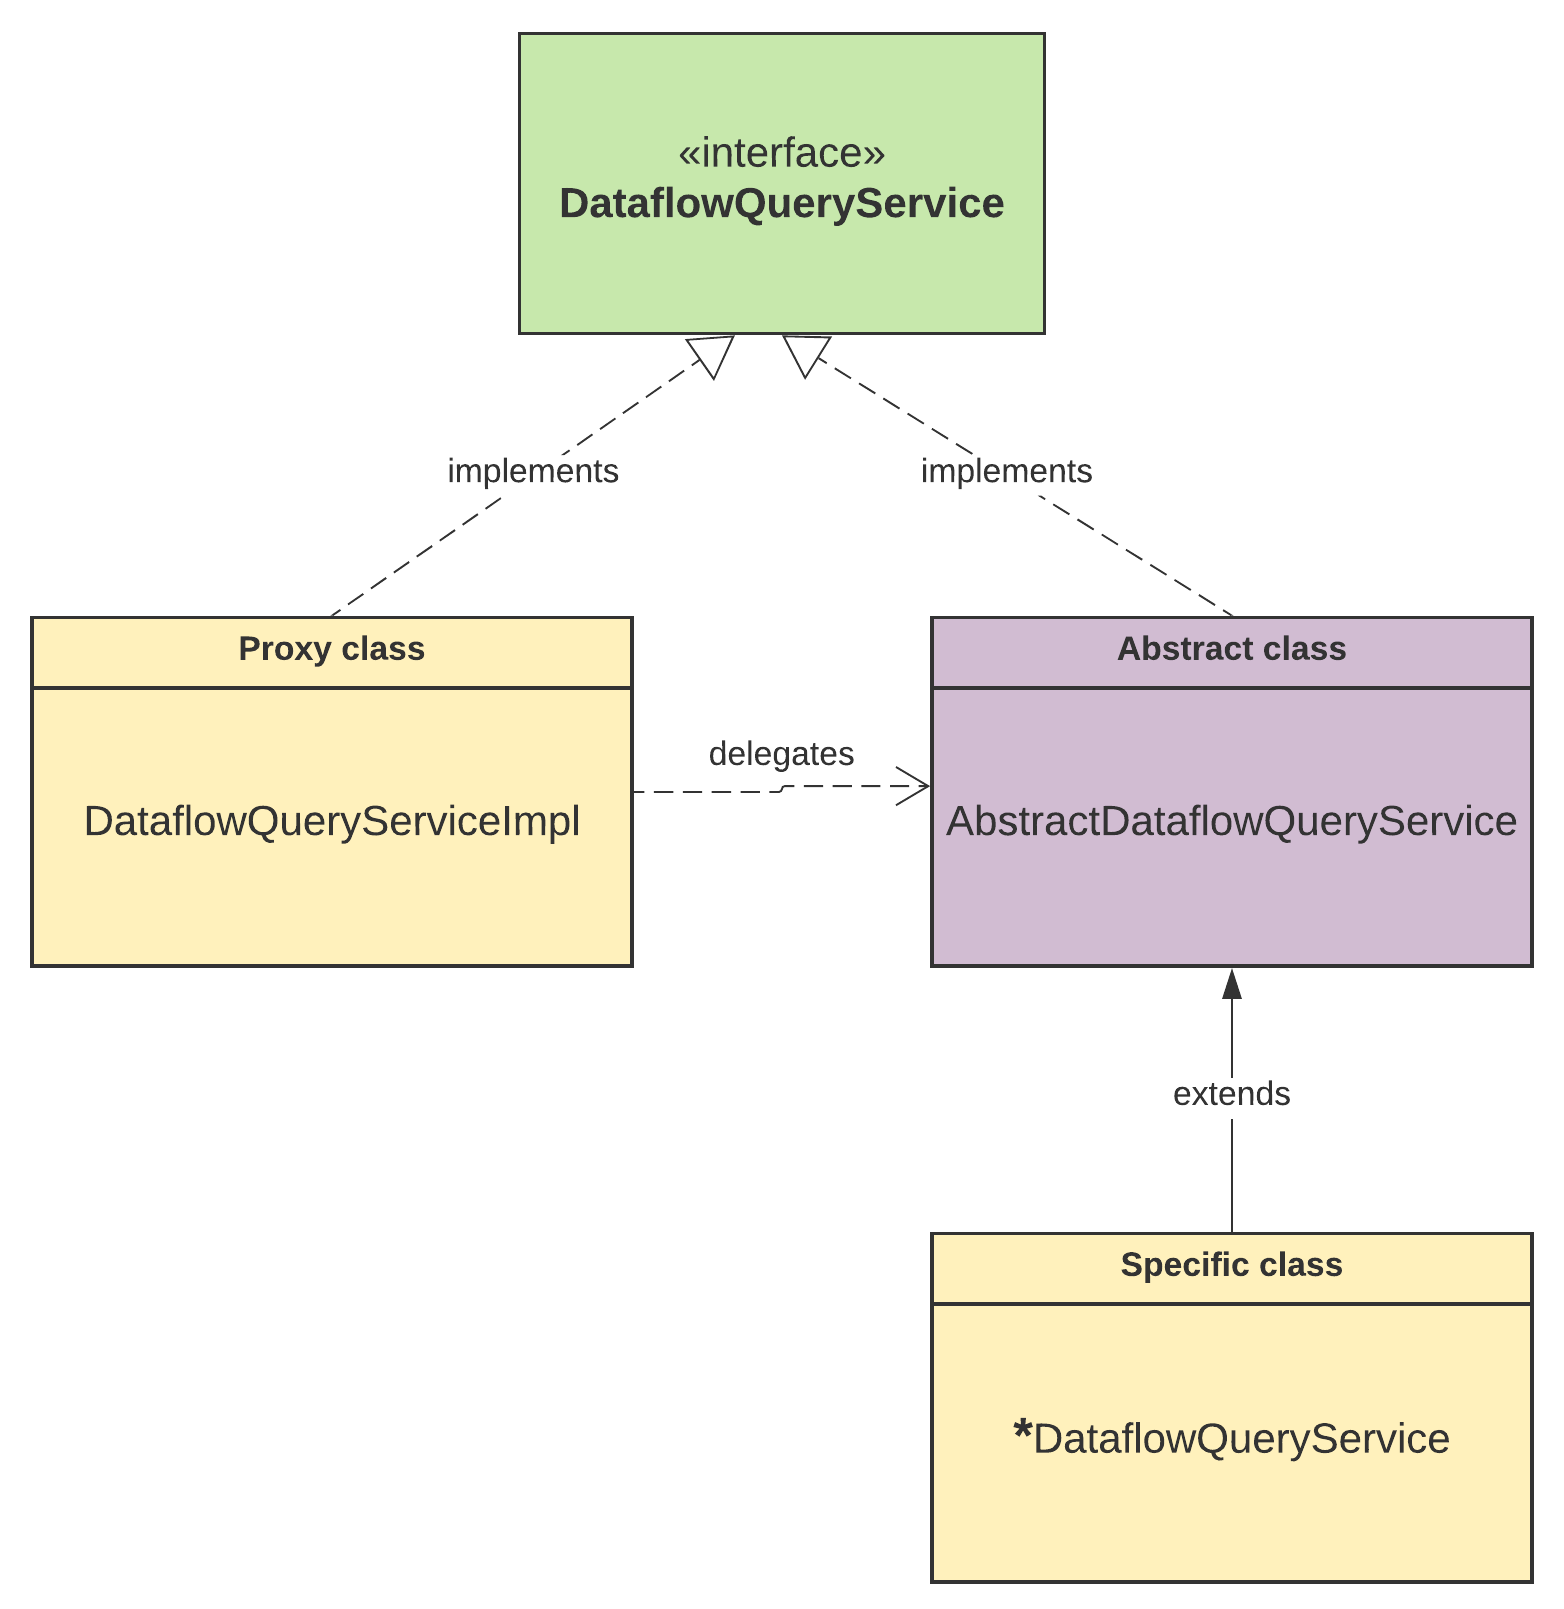
\includegraphics[width=1.0\textwidth]{img/cls.png}
\caption{A simplified class diagram of Dataflow Query Service}
\label{fig01:QS}
\end{figure}  


\texttt{DataflowQueryService} is a common interface that provides methods for client scanners for analyzing SQL queries or creating hierarchical database structures. This interface is implemented by:
\begin{itemize}
    \item Individual database query services that contain logic for providing data flows or hierarchical database structures.
    \item Proxy class called \texttt{DataflowQueryServiceImpl} that wraps all other individual query services. It is a classic implementation of a proxy class that chooses a specific query service based on information provided in the connection from the caller and delegates the operation.    
\end{itemize}

A simplified class diagram is depicted in figure~\ref{fig01:QS}.

% Description of language scanners, their composition, how they work
%- no DDL/dictionaries, only scripts
%- extraction is just a preparation of the input
%- analysis uses worklist algorithm, intermediate dataflow generator, common output
%- differences with database scanners
%- 
%---------------------
% SECTION
%---------------------
\section{Programming Language Scanners}

It might seem that analyzing all databases, ETL, reporting and analytic tools could yield a complete data lineage of an environment, but the fact is that these are not all data technologies that take part in data pipelines. There are also other applications, often developed by the companies themselves that engage in data processing. As these applications are unique, the only thing they have in common with other applications is the programming language used to write the source code. Therefore, the only universal way to analyze them is to perform the data flow analysis of the source code.
\par
Programming language scanners are one of the most complex scanners in Manta Flow. There are currently three of them: Bytecode scanner, C\# scanner and Python scanner. The scope of processes that can be expressed in a programming language is much greater and more complex compared to other data technologies. These scanners perform static code analysis to analyze data flows in the application and construct data lineage graph.
\par
Static code analysis is a method of analyzing source code without executing it. It involves examining the code's structure, syntax, and logic to observe certain properties. Often it is used to improve code quality and detect issues that could lead to runtime errors or security vulnerabilities, but it can have many other use-cases.
\par
There are other ways to analyze the code, but they are not suitable in the situations where Manta Flow is used. We cannot run the code for the analysis purposes, because it causes side effects (the pipeline would be executed). We also don't want to force the customers to modify the source code to record the events that are happening for the purposes of data lineage analysis, because often there are hundreds to thousands of code files that they want to analyze. It would be very labour intensive and minimizing labour is one of the reasons they use Manta Flow. We can only look at the code, so static analysis remains as the most feasible option.
\par
The goal of this static analysis is to find where data is read into the application, track it across all transformations and then find where it is written out. This proved to be a difficult task. There are several approaches for static code analysis, but none of them is aimed at data lineage, so a custom algorithm had to be developed. It uses symbolic analysis and an iterative approach along with multiple optimisations to produce limited results in a limited environment. These limitations are computing power, memory space and time. Manta Flow is expected to run in a common enterprise environment on a machine with a standard multi-core CPU, a reasonable RAM size (e.g. 32GB). Furthermore, the analysis is expected to end in the span of hours up to a few days. Due to that the output focuses on visualizing data reads and writes and data flows between them but it does not show details of intermediate transformations.

\subsection{Dataflow analysis of source code}

Let us describe how this analysis works in more detail. It will help us understand problems and solutions later in this work. All programming language scanners follow a similar workflow, but they implement each step in a little different way due to differences between the languages. Let us focus more on the details of Python scanner as it will be more relevant for the rest of this work. The structure of programming language scanners is also a bit different from other scanners, the core of the data flow analysis is performed by the Reader component as opposed to Dataflow Generator in other scanners. We shall explain why later in this section when more context is provided. A workflow diagram can be seen in figure~\ref{fig02:pythonWorkflow}.

\begin{figure}[ht]\centering
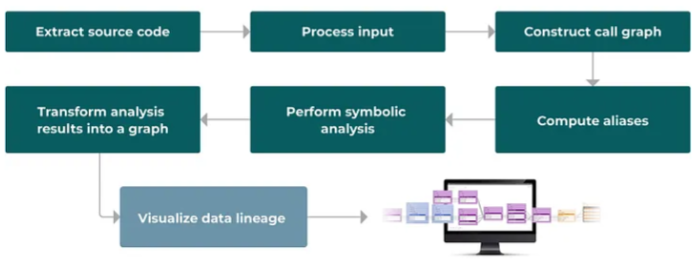
\includegraphics[width=1.0\textwidth]{img/python_workflow.PNG}
\caption{A simplified diagram of Python scanner workflow}
\label{fig02:pythonWorkflow}
\end{figure}  

Let us use the following simple Python program called \texttt{json\_to\_csv.py} shown in figure~\ref{fig:pythonSample} as an example. The program converts a JSON file to CSV format. Firstly, a JSON file is read using a built-in Python library \texttt{json}. Then, using a popular Python library for data manipulation called \texttt{pandas}, the contents of a JSON file are converted to a data frame, which is an abstraction of tabular data. Finally, the data frame is written to a file in CSV format. Clearly, the data flow in this program is pointing from the JSON file to the CSV file. Let us now take a look what happens inside the Python scanner with this program.

\begin{figure}[ht]
\begin{lstlisting}[language=Python] 
import pandas as pd
import json

# Loads json from file
def get_customer_data():
    with open("customer_data.json") as file:
        return json.load(file)

customer_data = get_customer_data()
df_customer = pd.json_normalize(customer_data)

df_customer.to_csv("customer_data.csv")
\end{lstlisting}
\caption{Sample Python program json\_to\_csv.py}
\label{fig:pythonSample}
\end{figure}

\subsubsection{Source code extraction}

The first step is source code extraction. Before the analysis can begin, all inputs need to be collected and prepared in the format they are expected to be in. The applications usually consist of the application code and of external libraries. The user only needs to provide the source code they wrote (so in our example only \texttt{json\_to\_csv.py}). The code of supported 3rd party libraries (\texttt{json} or \texttt{pandas}) that are used is added by the scanner as it stays the same across different use cases. When the files are collected, an extraction configuration is generated which captures the structure of the input and allows the user to specify which functions or modules should be considered as analysis entry point.
\par
Analysis entry point is the routine that shall be considered as a starting point of a program execution. Usually, it can be the \texttt{main} method in Java or C\# or the module containing \texttt{\_\_main\_\_} block in Python, but in general it can also be any other function, method or module. This defines the starting point of the analysis and from that point function invocations and variable assignments are tracked. In our example, it would be the \texttt{json\_to\_csv.py} module.
\par
Source code extraction is a standalone step and represents metadata extraction for programming language scanners. It is a part of Extractor component.

\subsubsection{Input processing}

Now we are moving to Reader component of Python scanner. In this initial step of dataflow analysis, the extracted inputs are read from file system and pre-processed. In Python, this involves parsing of the source code into a convenient internal representation. There are a couple data structures that need to be created in this step which are used in the following ones.
\par
One of these structures is class hierarchy, which helps with the detection of invocation targets (this is implemented in Bytecode and C\# scanners, but not yet in Python scanner). The other, more important for the algorithm is \textit{call graph}. It captures caller-callee relationship between executables (functions, methods, modules) in the application. A caller is the executable that invokes another executable in its body, a callee is the executable that is being invoked by another executable. Call graph helps to find which other executables need to be analyzed again after the analysis of one, because its result might influence the callers and callees. This will be explained in more detail later.

\subsubsection{Alias analysis}

Aliases are different expressions that might reference the same value. It is important to analyze assignments in the application to resolve these aliases, because a value assigned into one of these expressions has to be propagated into all aliases. Similarly, if a value in an expression is modified, so it is in all of the aliases. An alias could be understood as a synonym to a reference, but it tracks a few more cases than just references. Figure~\ref{fig:alias} shows how an alias can be created.

\begin{figure}[ht]
\begin{lstlisting}[language=Python] 
foo = "Hello World!
bar = foo # bar now aliases the same value as foo does
\end{lstlisting}
\caption{An example of an alias}
\label{fig:alias}
\end{figure}

\subsubsection{Symbolic analysis}

With all the preparatory steps done, we now have everything ready for \textit{symbolic analysis}, which is the core of the data flow analysis. It is based on an iterative analysis of executables and propagating data flows as defined by assignments and function invocations.
\par
\textit{Data flows} (or shortly just \textit{flows}) represent a meaningful data lineage information in the source code. We can split flows into two groups. Metadata flows are flows that represent any form of data flowing in the program, for example data read from a database, file etc. These do not represent a concrete value, but rather its meta representation, e.g. a column in a database table. The other group are value flows which track a possible runtime value of a variable. Even though we already mentioned that we do not execute the code, we need to track string values in code, because they can be used for identification of resources, such as file or column names. In our example, these values contain names of the files that data is read and written to.
\par
To find the data flows, the algorithm analyzes executable invocations. An invocation consists of the body of an executable (instructions) and arguments. The arguments contain the flows for function parameters that the function was invoked with and in Python also flows of global variables, which can be also accessed. If the same function is called with two different sets of arguments, they are two different invocations.
\par
The invocations are analyzed in an order defined by a worklist (an enhanced queue) in a loop until it is empty. At first, it contains the entry point. At the beginning of each loop, the first invocation is removed from the worklist and analyzed. When an invocation is analyzed, a so-called \textit{executable summary} is computed. This summary contains flows of expressions at each instruction in the executable. Consider this part of the example code:
\begin{verbatim}
customer_data = get_customer_data()
\end{verbatim}
Firstly, the flow of the return value of \texttt{get\_customer\_data()} is resolved and assigned to its corresponding expression. Next, this flow is looked up and assigned to the flow of the expression \texttt{customer\_data} etc. When the processing of an invocation is finished, a complete executable summary is stored in a cache.
\par
To keep the algorithm going, we need to add new invocations into the worklist. When the analysis finds an instruction representing an invocation, it is not processed recursively. After all, the point of using a worklist is to avoid recursion which can cause stack overflow very easily. Instead, it has to be looked up. At this point, it matters whether the invoked function comes from application code or from a library. For application functions, the summary of the invocation is looked up in the cache. If it has been already computed, it is used to resolve the flow of the return value. If not, it is added to the worklist and will be computed later.
\par
If the function comes from library code, it is not analyzed at all. The goal is to analyze application source code, not the code of the libraries. Library code is known to us in advance, so instead of analyzing them instruction after the instruction, we can directly create the returned data flow. Python scanner contains many data flow plugins which implement flow propagations for different libraries and they are the main area of improvement. Of course, it is not possible to cover each function in each library, so plugin development is aiming at those libraries that are most widely used. If such function is not covered by a plugin, there is a fallback \textit{identity handler}. It propagates flows of the arguments to the return value. It is not the most accurate propagation, but it keeps the algorithm going.
\par
Getting back to how worklist is filled, new invocations of application executables are added at its end. When there were such invocations, the current invocation is also added to the worklist so when the new invocations are computed, the current invocation could be updated with their summaries. Also, if its summary has changed from the last time it was computed, it is necessary to recompute its callers, that is, invocations that called it. They might not be anymore in the worklist, but the changed summary of the current invocation may have an effect on them so they need to be recomputed. We can easily find callers from the call graph that was computed in input processing phase.
\par
When there are no more changes to the summaries, the algorithm has reached a stable point and the symbolic analysis is considered to be over.

\subsubsection{Output transformation}

The result of symbolic analysis contains a lot of executable summaries. That is however not the result we can call a data lineage graph. We need to transform the result of data flow analysis to a data lineage graph. During the symbolic analysis, when we come across an invocation that represents a data input or an output such as database select or file write, on top of propagating the flow in the summary we also register it. Then, to transform the result into a graph, all we need to do is to iterate over the summaries and find the registered flows.
\par
Flows are implemented in such a way that they track their origin, so an output flow contains the source of the data that is written out. Not all output flows contain a valid input, so some filtering has to be applied during the transformation, but eventually nodes for inputs and outputs are created along with corresponding edges. It might seem that we only need to register output flows and we can find the input flows in them, but we also register input flows in case there is an unused one (an unused input can still cause an error during program execution).
\par
The result of the transformation is called a \textit{connector output}. It is not yet a Manta graph, but rather a boilerplate for creating it. It contains the information about nodes that should be created and which nodes should be connected with edges. The reason for it is that all programming language scanners create a very similar output so creating a Manta graph from such output can be implemented once and used by all scanners.

\subsubsection{Generating Manta graph}

\begin{figure}[ht]\centering
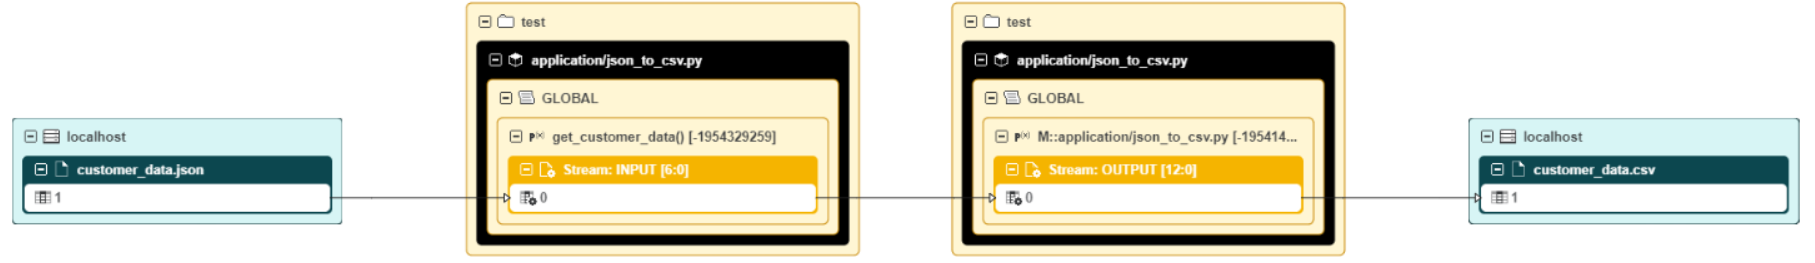
\includegraphics[width=1.0\textwidth]{img/json_to_csv.PNG}
\caption{Visualization of the data lineage from the example}
\label{fig:lineage}
\end{figure}  

Finally, the last step of the analysis is to generate a Manta graph from a connector output. This happens in Dataflow Generator component and as already mentioned, there is one common generator for all programming language scanners. All analytic work has already been done, so the generator simply reads the connector output and creates corresponding nodes in the Manta graph. Should there be any SQL queries, it uses Dataflow Query Service to resolve them. The graph that is created is considered the output of the scanner. A visualization of the data lineage graph created from the \texttt{json\_to\_csv.py} example can be seen in figure~\ref{fig:lineage}.